\documentclass[tikz,border=10pt]{standalone}
% No extra TikZ libraries are needed.
\begin{document}
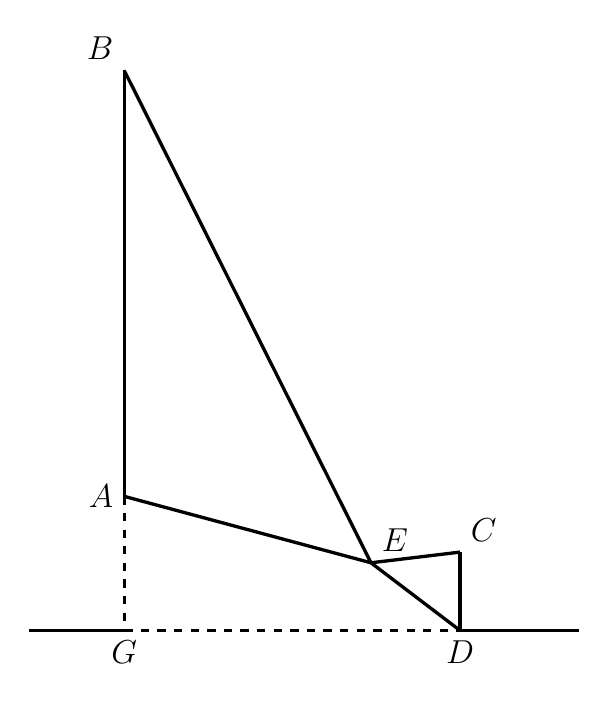
\begin{tikzpicture}[line join=round, line width=1.2pt,
  lbl/.style={font=\fontsize{12}{14.4}\selectfont}]
  % Scale: s = 0.015066 cm/px, centred on ink bbox centre (255.5, 302) px
  % Points (x_t = (px-255.5)*s, y_t = (302-py)*s)
  \coordinate (B) at (-2.2825, 3.5556);   % px (104,66)
  \coordinate (A) at (-2.2825, -1.8531);  % px (104,425)
  \coordinate (G) at (-2.2825, -3.5556);  % px (104,538)
  \coordinate (D) at (1.9812, -3.5556);   % px (387,538)
  \coordinate (C) at (1.9812, -2.5612);   % px (387,472)
  \coordinate (E) at (0.8512, -2.6968);   % px (312,481)
  \coordinate (L) at (-3.4878, -3.5556);  % px (24,538)
  \coordinate (R) at (3.4878, -3.5556);   % px (487,538)

  % Solid vertical B-A
  \draw (B) -- (A);
  % Dashed A-G
  \draw[dashed] (A) -- (G);
  % Solid A-E, B-E, E-C, C-D, E-D
  \draw (A) -- (E);
  \draw (B) -- (E);
  \draw (E) -- (C);
  \draw (C) -- (D);
  \draw (E) -- (D);
  % Dashed horizontal G-D
  \draw[dashed] (G) -- (D);
  % Solid baselines
  \draw (L) -- (G);
  \draw (D) -- (R);

  % Labels
  \node[above left, lbl] at (B) {$B$};
  \node[left, lbl] at (A) {$A$};
  \node[above right, lbl] at (E) {$E$};
  \node[above right, lbl] at (C) {$C$};
  \node[below, lbl] at (G) {$G$};
  \node[below, lbl] at (D) {$D$};
\end{tikzpicture}
\end{document}